\documentclass[11pt, letterpaper]{article} 

%%%% ----- PACKAGES ---- %%%%

% Fonts & Colors
\usepackage[utf8]{inputenc}
\usepackage[T1]{fontenc}
\usepackage{lmodern}
\usepackage[svgnames,usenames,dvipsnames,x11names,table]{xcolor}
\usepackage{microtype}

% Math 
\usepackage{amsmath,amsthm}
\usepackage{amsfonts,eucal,amssymb,amscd,empheq,bm,mathtools}
\usepackage{mathrsfs}
\usepackage{calc} 

% Tikz & boxes
\usepackage{tikz}
\usepackage[framemethod=tikz]{mdframed}
\usepackage{framed}

% interface for floats (Figures/Tables), allows 'H' option
\usepackage{float}

% expanded footnote package
\usepackage{bigfoot}

% refinements 
\usepackage{setspace}
\usepackage{graphicx}
\usepackage[normalem]{ulem}
\usepackage{fancyhdr}
\usepackage[pdftex]{hyperref}
\usepackage{url}

%\usepackage{amsmath, amsfonts, amsthm}
%\usepackage[svgnames,table]{xcolor}
\usepackage[hang, small, labelfont=bf, up, textfont=it]{caption}
\usepackage{booktabs} 

\usepackage{enumerate}
\usepackage{listings}
\usepackage{marginnote}
\usepackage{mparhack}

\usepackage{longtable}
\usepackage[labelfont=bf,indention=0cm]{caption}
\usepackage{subcaption}

\usepackage{verbatim}
\usepackage[makeroom]{cancel}

\usepackage{geometry}
\usepackage[most]{tcolorbox}
\usepackage{tabularx}

\usepackage{bookmark}
\usepackage[lite]{amsrefs}
\usepackage{arydshln}

\usepackage{booktabs}
\newcounter{lecnum}
\usepackage{nicefrac}
\usepackage{tcolorbox}
\tcbuselibrary{theorems}

\usepackage{enumitem} 
\setlist{noitemsep} 
\usepackage{sectsty} 
\allsectionsfont{\usefont{OT1}{phv}{b}{n}}

\makeatletter
\def\@seccntformat#1{\csname the#1\endcsname.\quad}
\makeatother

\usepackage{geometry}
\geometry{
	top=0.75in,
	bottom=0.75in,
	left=1.5in,
	right=1.5in,
	includehead,
	includefoot,
	%showframe, 
}

\hypersetup{pdftex, colorlinks, citecolor=blue, filecolor=blue, linkcolor=blue, urlcolor=blue}

\pagestyle{fancy}
\PassOptionsToPackage{normalem}{ulem}
\makeindex
\setlength{\headheight}{12pt}


\setlength{\columnsep}{7mm} % Column separation width
\usepackage[T1]{fontenc}
\usepackage[utf8]{inputenc} 
\usepackage{XCharter} 
\usepackage{fancyhdr} 
\pagestyle{fancy} 

\renewcommand{\headrulewidth}{0.0pt} 
\renewcommand{\footrulewidth}{0.0pt}

%\renewcommand{\footnotesize}{\scriptsize}
\setlength{\skip\footins}{10pt}

\usepackage[numbered,framed]{matlab-prettifier}
\lstset{style= Matlab-editor,
    basicstyle = \mlttfamily\footnotesize,
    breaklines=false,
    %backgroundcolor=\color{light-gray},
    numbersep=5pt,
    xleftmargin=.25in,
    xrightmargin=.25in 
} 

%\usepackage[parfill]{parskip}
%\setlength{\parskip}{4pt} 
\setlength{\parindent}{0pt}

% format/layout adjustments
\newcommand{\n}{\vskip 6pt \noindent}
\newcommand{\nn}{\vspace{8mm} \noindent}
\newcommand{\ns}{\vspace{8mm}}

% for adjustwidth environment
\usepackage[strict]{changepage}

% environment derived from framed.sty: see leftbar environment definition
\definecolor{formalshade}{rgb}{0.95,0.95,1}
\definecolor{darkBlue}{RGB}{25,25,112}

\newenvironment{formal}{%
\small
  \def\FrameCommand{%
    \hspace{1pt}%
    {\color{darkBlue}\vrule width 2pt}%
    {\color{formalshade}\vrule width 4pt}%
    \colorbox{formalshade}%
  }%
  \MakeFramed{\advance\hsize-\width\FrameRestore}%
  \noindent\hspace{-4.55pt}% disable indenting first paragraph
  \begin{adjustwidth}{}{7pt}%
  \vspace{-12pt}
  \vspace{2pt}\vspace{2pt}%
}
{%
  \vspace{2pt}\end{adjustwidth}\endMakeFramed%
}

\usepackage{sectsty}
\subsectionfont{\normalfont\itshape}


% Removes the section number from the header when \leftmark is used
\renewcommand{\sectionmark}[1]{\markboth{#1}{}} 

\usepackage{titlesec}
\titleformat{\subsubsection}{}{\thesubsubsection}{1em}{\itshape}



%\nouppercase\leftmark % Add this to one of the lines below if you want a section title in the header/footer

% Headers/ footers
\lhead{}
\chead{} 
\rhead{}

\lfoot{} 
\cfoot{} 
\rfoot{} % Right footer, "Page 1 of 2"

\fancyfoot[C]{\fontsize{9}{12} \selectfont \vspace{12pt} \textit{\footnotesize{\thepage}}}

% Page style for the first page with the title
\fancypagestyle{firstpage}{ 
	\fancyhf{}
	\renewcommand{\footrulewidth}{0pt}
}

%----------------------------------------------------------------------------------------
%	TITLE SECTION
%----------------------------------------------------------------------------------------

\newcommand{\authorstyle}[1]{{\large\usefont{OT1}{phv}{b}{n}\color{DarkRed}#1}} 
\newcommand{\institution}[1]{{\footnotesize\usefont{OT1}{phv}{m}{sl}\color{Black}#1}}
\usepackage{titling} 
\newcommand{\HorRule}{\noindent \color{DarkGoldenrod}\rule{\linewidth}{0pt}} 

\pretitle{
\centering
	\vspace{-5pt} 
	\HorRule\vspace{10pt} 
	\fontsize{24}{28}\usefont{OT1}{phv}{m}{n}\selectfont 
	\color{DarkRed} 
}
\posttitle{
\centering
\par\vskip2pt
} 

\preauthor{} 
\postauthor{ 
	\vspace{0pt} 
	\par\HorRule
	%\vspace{20pt} 
	\vspace{-1cm} 
}


\theoremstyle{break}
\newtheorem{example}{Example}[section]

\mdfdefinestyle{mystyle}{
  hidealllines=true,
  leftline=true,
  innerleftmargin=10pt,
  innerrightmargin=10pt,
  innertopmargin=10pt,
}


\newmdtheoremenv[style=mystyle]{example2}{Example}




\theoremstyle{definition}
\newtheorem{defnn}{Definition}
\newtheorem*{tst*}{}
\newmdtheoremenv[style=mystyle]{defnn2}{Definition}

\newtheorem*{Alg*}{Algorithm}
\newtheorem*{rmk*}{Remark}
\newtheorem*{thm}{Theorem}
\newcommand{\Recall}{\vspace{4mm}\noindent \bd{\ul{Recall}}}
\newcommand{\Note}{\vspace{4mm}\noindent \bd{\ul{Note}}}
\newcommand{\Question}{\vspace{4mm}\noindent \bd{\ul{Question}}}

\newcommand{\Problem}[1]{\vspace{4mm}\noindent {\large\bd{\ul{Problem #1}}}}



		%%%%%%%%%%%%%%%%%%%%%%%%%%%%%%%% DEFINITIONS  %%%%%%%%%%%%%%%%%%%%%%%%%%%%%%%%%%%

\theoremstyle{definition}
\newtheorem{quest}{Question Set:}
\newtheorem{deliv}{Deliverable}



%%%%%%      MATH ENVIRONMENT      %%%%%%%%

% align
\newcommand{\eq}[1]{\begin{align*}#1\end{align*}}

% tags
\newcommand{\tagit}[1]{\tag{\it{#1}}}
\newcommand{\tagitb}[1]{\textcolor{blue}{\tag{\it{#1}}}}



% font
\newcommand{\ul}[1]{\underline{#1}}
\renewcommand{\it}[1]{\textit{#1}}
\newcommand{\bd}[1]{\textbf{#1}}
\newcommand{\bul}[1]{\textbf{\ul{#1}}}
\newcommand{\bit}[1]{\textbf{\textit{#1}}}



% shortcuts for letters, symbols & etc
\def\nhat{\bm{\hat{n}}}

\newcommand{\Z}{{\mathbb{Z}}}
\newcommand{\R}{{\mathbb{R}}}
\newcommand{\N}{{\mathbb{N}}}
\newcommand{\F}{{\mathcal{F}}}
\newcommand{\C}{{\mathcal{C}}}
\newcommand{\W}{{\mathcal{W}}}
\newcommand{\E}{{\mathcal{E}}}
\newcommand{\A}{{\mathcal{A}}}
\newcommand{\X}{{\mathbb{X}}}


% colors
\colorlet{shadecolor}{Red!5}
\colorlet{framecolor}{Red!1}
\definecolor{dkred}{RGB}{165,0,0}

%%%%% BOXED EQUATIONS %%%%%%%
\newcommand*\widefbox[1]{\fbox{\hspace{2em}#1\hspace{2em}}}

% shading
\newenvironment{frshaded}{
 \def\FrameCommand{\fboxrule=\FrameRule\fboxsep=\FrameSep \fcolorbox{framecolor}{shadecolor}}%
 \MakeFramed{\FrameRestore}}%
 {\endMakeFramed}

 \newenvironment{frshaded*}{%
 \def\FrameCommand{\fboxrule=\FrameRule\fboxsep=2\FrameSep \fcolorbox{framecolor}{shadecolor}}%
 \MakeFramed{\advance \hsize - \width \FrameRestore}}%
  {\endMakeFramed}



% horizontal & vertical lines
\newcommand*{\vertbar}{\rule[-1ex]{0.5pt}{2.5ex}}
\newcommand*{\horzbar}{\rule[.5ex]{3ex}{0.5pt}}

%%%%%%      SHORTCUTS     %%%%%%%%
\newcommand{\dt}{{\Delta t}}
\newcommand{\dx}{{\Delta x}}
\newcommand{\idt}{{\frac{1}{\Delta t}}}
\newcommand{\idx}{{\frac{1}{\Delta x}}}
\newcommand{\dtdx}{\frac{\Delta t}{\Delta x}}
\newcommand{\dxdt}{\frac{\Delta x}{\Delta t}}

\newcommand{\Qin}{{Q_{i}^{n} }}
\newcommand{\Qini}{{Q_{i}^{n \+ 1} }}
\newcommand{\Qimi}{{Q_{i}^{n \- 1} }}
\newcommand{\Qinp}[1]{{Q_{i}^{n \+ #1} }}

\newcommand{\qx}{q_{,x}}
\newcommand{\qxx}{q_{,x,x}}
\newcommand{\qt}{q_{,t}}
\newcommand{\qtt}{q_{,t,t}}

\newcommand{\ordii}{\ord( \dx^2)}
\newcommand{\ordiii}{\ord( \dx^3)}

\renewcommand{\uplus}{u^{\+}}
\newcommand{\uminus}{u^{\-}}

\newcommand{\Fii}[2]{\F_{ i \+ \h}^{n \+ \h}}
\newcommand{\Fnn}[2]{\F_{ #1}^{#2}}
\newcommand{\FF}{\Scale[1.4]{\mathscr{F}}}

\newcommand{\sumN}{\sum_{i \= 1}^{N} }
\newcommand{\summ}{\sum_{p \= 1}^{m} }
\newcommand{\suminf}{\sum_{i \= -\infty}^{\infty} }

\newcommand{\ord}{{\mathcal{O}}}
\newcommand{\into}{\rightarrow}

\newcommand{\stari}{\raisebox{.2\height}{\scalebox{0.9}{\ensuremath{\hspace{0.25mm} \star}}}}


\newcommand{\lp}{\lambda^{(p)}}

%% SUPERSCRIPTS
\newcommand{\soln}{\it{sol}\textsuperscript{\ul{\it{n}}}}
\newcommand{\Soln}{\it{Sol}\textsuperscript{\ul{\it{n}}}}
\newcommand{\eqn}{\it{eq}\textsuperscript{\ul{\it{n}}}}
\newcommand{\Eqn}{\it{Eq}\textsuperscript{\ul{\it{n}}}}

\newcommand{\st}{\textsuperscript{\ul{\it{st}}} }
\newcommand{\nd}{\textsuperscript{\ul{\it{nd}}} }

% create a matrix: use &, \\ as normal
\newcommand{\mtx}[1]{\left(\begin{matrix}#1\end{matrix}\right)}


%%%%% EQUATIONS  %%%%%%

\newcommand{\burgers}{\eq{  q_{,t} + \Big( \h q^2 \Big)_{,x} = 0 }} 			% Burger's Eqn






%%%%% GRAPHICS %%%%%
\newcommand{\gfxi}[1]{
\vspace{3mm}
  \begin{center}
    \begin{figure}[h!]
    \includegraphics[height=45mm]{#1}
    \end{figure}
  \end{center}
}

\newcommand{\gfxii}[2]{
\vspace{3mm}
  \begin{center}
    \begin{figure}[h!]
    \includegraphics[height=#1mm]{#2}
    \end{figure}
  \end{center}
}

% figure + equation/text, side by side
\newcommand{\gfxss}[2]{
\vspace{3mm}
\noindent\begin{minipage}{.45\textwidth}
 	\centering
   		\includegraphics[height=45mm]{#1}
  		\label{fig:figure}
\end{minipage}
\begin{minipage}{.45\textwidth}
#2
\end{minipage}
}

 
\graphicspath{{./gfx/}}
\usepackage[boxed]{algorithm2e}
\usepackage{xfrac}

\title{ \textsc{Prelab Exercise 2: \\ Extended Surfaces} \\ {\large  \color{darkgray} ME 436 Heat Transfer}}

\begin{document}
\date{}
\maketitle
\thispagestyle{firstpage} 

\section*{Introduction}

The primary objective of this experiment is to theoretically and experimentally study an \it{extended surface} subjected to varying environmental conditions. More specifically, a heated cylindrical rod, lined with evenly-spaced thermocouples,  will be examined under passive, medium, and high air flow rates - simulating free, medium, and high convective conditions. The temperature distributions and heat transfer rates will be calculated using three separate models; the most accurate of which will ultimately be selected. Finally, performance metrics are used to assess the effectiveness and efficiency of the extended rod for use as a fin.
\n
This pre-lab assignment will act as a guide towards creating a mathematical model before attending lab --  saving critical in-class time for performing experiments and analyzing data. 

\section*{Prerequisites}
Before attempting this pre-lab assignment, it is imperative that you:
{\small
\begin{itemize}
    \item Review \bit{textbook section 3.6}, particularly \bit{Table 3.4} \it{(pg. 161)},
    \item Review \bit{experiment procedures}, and
    \item Watch the \bit{pre-lab videos} on Blackboard (Bb).
\end{itemize}
}


\section*{Getting Started}
First, be sure to download the starter code from Blackboard (Bb), and \textit{extract} (unzip) its contents to the directory in which you wish to complete the exercise\footnote{\textit{Note: when using the Heat Transfer Lab computers, you \ul{must} extract your code to the local hard drive: \texttt{C:/temp/}, NOT to the server (ie., Desktop, Group Folder, \&, etc.)}}. Before attempting, make sure that you have completed all of the \textit{prerequisites} below.

\subsection*{Files included in this exercise:}
Once you have unzipped the contents of the starter package, you should see the following files:

\begin{itemize}
\renewcommand\labelitemi{-- }
   \item \bd{\texttt{ex2.m}}
    \item \texttt{/lib}
    \item  \texttt{caseA.m}
\renewcommand\labelitemi{[$\star$]}
    \item \texttt{caseB.m}
    \item \texttt{caseD.m} 
    \item \texttt{calc\_eta.m} 
    \item \texttt{calc\_epsilon.m} 
\renewcommand\labelitemi{[$\dag$]}
    \item \texttt{ex2\_rad.m} 
    \item \texttt{calc\_rad.m}
    \item \texttt{calc\_conv.m}  
\end{itemize}

\noindent
$\star$ indicates files that you will need to complete.\\
$\dag$ indicates files that are optional (at this time).

\n
Throughout this pre-lab exercise, you will be using the script \bd{\texttt{ex2.m}}, but will only be required to edit \bit{one section}, in which you will need to enter material properties, defined in the \bit{laboratory procedures}.


\setcounter{section}{-1}
\section{Environment Setup}
Before we can get started, we need to setup our MATLAB environment properly. As always, if using the laboratory computers, be sure to be running your code from the \texttt{C:\textbackslash temp} directory, and also make sure you have unzipped your code properly. Otherwise you may receive `\texttt{./lib not found}' errors.

\subsection{MATLAB Script Outline}

Once your environment is setup, open the file named \bd{\texttt{ex2.m}} and read the instructions at the top of the script. In short, this script will plot your data and fit the math models described in \bit{Table 3.4} to your collected dataset. A brief outline of the script is shown below. The essential parts of this assignment are highlighted in red.
\IncMargin{1em}
\begin{algorithm}[ht]
\caption{Extended Surface Model}
\SetKw{Set}{Set: }
\SetKw{Call}{Call: }
\SetKw{Load}{\emph{load: }}
\SetKwComment{cc}{\% }{ }
\SetKw{Plot}{Plot: }
\SetKw{Print}{Print: }

    \emph{clear; close all}\;
    \Set{path to data}\;
    \Set{properties}\;
    \BlankLine
    \For{$i = 1$ \KwTo 3,}{\label{forins}
      \Load{excel dataset(i)}\;
      \Indp \texttt{[dat]} $\leftarrow$ \texttt{xlsread(path)}\;
      \Indm \Set{average SS temps}\;
      \Indp\texttt{[Tm]} $\leftarrow$ \texttt{mean(dat)}\;
         \BlankLine
          \Indm\Set{theoretical temps}\;
       \Indp $[T_A, q_A ]\leftarrow $ \texttt{caseA()}\;
        $[T_B, q_B] \leftarrow $ \textcolor{dkred}{\texttt{caseB()*}}\;
        $[T_D, q_D] \leftarrow $ \textcolor{dkred}{\texttt{caseD()*}}\;
         \BlankLine
         \Indm \Set{performance}\;
        \Indp $ \eta  \leftarrow $ \textcolor{dkred}{\texttt{calc\_eta()*}}\;
         $ \epsilon  \leftarrow $ \textcolor{dkred}{\texttt{calc\_epsilon()*}}\;
     }
     \Plot{ $T_{A,B,D}$ vs. $T_{m}$}\;
     \Print{ $q$ \& $\epsilon$, $\eta $} to screen\;
\end{algorithm}

\n
\n

Now, in the MATLAB editor, scroll down to the \texttt{SETUP} section. This portion of the script is where the paths to our data are set. More specifically, \texttt{pDIR} is the \it{folder} in which \bit{all three datasets} are stored. Then, for each dataset you will need to enter three critical pieces of information:
\begin{enumerate}
    \item Filename,
    \item Convection coefficient, $h$,
    \item Title to describe the data once plotted
\end{enumerate}

\n
Examples are provided to you using the sample dataset:

\n
\begin{lstlisting}[numbers=none]
% set 1
fname{1,1} = 's1_h9.xlsx';
h(1) = 9;    % [W/m^2 C]
titles{1,1} = 'Temperature Distribution: h = 9 [W/m^2 C]';

% set 2
fname{1,2} = 's3_h30.xlsx';
h(2) = 30;   % [W/m^2 C]
titles{1,2} = 'Temperature Distribution: h = 30 [W/m^2 C]';

% set 3
fname{1,3} = 's5_h40.xlsx';
h(3) = 40;    % [W/m^2 C]
titles{1,3} = 'Temperature Distribution: h = 40 [W/m^2 C]';
\end{lstlisting}

\n
Here, it is easiest to simply replace the Excel sheet titles with your own data (be sure that your data has been moved to the \texttt{./data} folder).

\begin{center}
\begin{tcolorbox}[enhanced, width=14cm, size=tight, top=-2mm, colback=red!5, colframe=black!50!white, boxrule=0.25pt, boxsep=2mm]
\n
{\small
\bit{Note:} - When performing the experiment, make sure you have \bit{all three sets of data} collected before running this script.
}
\end{tcolorbox}
\end{center}


\section{Input Properties}

Now, we must input a few properties from the experiment procedures.

\begin{lstlisting}[numbers=none]
%% =========== Part 1: Input Properties ============= 
% Now, using the procedures document for reference, fill in the necessary
% information below
\end{lstlisting}

First, we \it{define} a few \texttt{global} variables. These are special variables that once set, will \textit{always} be available to us. That is, we don't need to pass them in/out of functions:
\begin{lstlisting}[numbers=none]
% set globals
global D k P L Ac Af T_inf
\end{lstlisting}

Now, we arrive to the \it{fin properties} section. Here you must replace the incorrect values or provide the correct equation (as appropriate):
\n

\n
\begin{lstlisting}[numbers=none]
% Fin Properties **FIX ME**
D = 1; %???                      % (Diameter) [m]
k = 1; %???                      % (Conductivity, Brass) [W/m C]
P = pi * D;                      % (Perimeter) [m]
L = 1; %???                      % (Length of fin) [m]
Ac = 1; %???                     % (Cross Sectional Area) [m^2]
Af = pi * D * L;                 % (Fin Surface Area) [m^2]

% Set Tinf -- as measured in lab
T_inf = 22.5;     % [C]
\end{lstlisting}

\n
\bit{Note:} The \texttt{Ac} and \texttt{Af} values refer to the \it{cross-sectional area} and \it{total fin surface area}, respectively. These also need to be set correctly. Once this is done, we can move on to the main loop.

\n
Now, when you're ready to continue, comment out the following line:

\n
\begin{lstlisting}[numbers=none]
% remove break
break_msg; dbstack; return;
\end{lstlisting}


\section{Plotting Loop}

This section now uses a simple \texttt{For-Loop} to process each data set automatically. While there are six stations in the lab, this assumes only \bit{\ul{three} are being processed at once.}
\n
As you walk through the inner-workings of the main loop, much of this should look familiar. You do not need to do anything here, but be sure to understand what is being done.

\n
\subsection{Plotting: Cases A, B, D}

However, once we get down to the following lines:
\n
\begin{lstlisting}[numbers=none]
% The fin excess temperatures
theta_x = Tm - T_inf;
theta_b = Tb - T_inf;
\end{lstlisting}

We are now ready to set our \it{theoretical} temperature distributions, as defined by three boundary conditions (BCs) at $(x=L)$, shown in \bit{Table 3.4}.

\begin{itemize}
    \item [--] \bit{Case A}: Convective BC,
    \item [--] \bit{Case B}: Adiabatic BC,
    \item [--] \bit{Case D}: Infinite Length BC.
\end{itemize} 

Functions for each of these cases are implemented in the code below:
\n
\begin{lstlisting}[numbers=none]
% m & M
M = sqrt((h(ii) * P * k * Ac)) * theta_b;
m = ((h(ii) * P) / (k * Ac))^0.5;
mL = m * L;
h_mk = h(ii)/(m*k);

% Case A
[TA, qA(ii)] = caseA(x, theta_b, m, M, h(ii));

% Case B
[TB, qB(ii)] = caseB(x, theta_b, m, M);

% Case D
[TD, qD(ii)] = caseD(x, theta_b, m, M);
\end{lstlisting}

\n
Here, we are setting the values from \bit{Table 3.4 from the textbook}. In summary, we are now inserting the equations for the \it{temperature distribution}, $T(x)$ and the \it{heat rate}, $q_f$.  The quantities \texttt{m} \& \texttt{M} have already been defined. What still needs to be done is for you to complete \bit{Cases B and D}; Case A has already been completed as an example.
\n
To complete this portion of the exercise, open the files \bit{\texttt{caseB.m}} \& \bit{\texttt{caseD.m}} and insert the correct equation(s) to allow the function to execute properly.
\n


\begin{center}
\begin{tcolorbox}[enhanced, width=14cm, size=tight, top=-2mm, colback=red!5, colframe=black!50!white, boxrule=0.25pt, boxsep=2mm]
\n
{\small
\bit{Note:}
\begin{itemize}
    \item The function is provided with the following input quantities: \texttt{x, theta\_b, m, M}. Hence, you \bit{do not} need to define them, just \it{use} them. \bit{See \texttt{caseA.m} as an example.}
    \item In addition, the \bit{global} values are available for you to use as well, you do not need to define them. \bit{See \texttt{caseA.m} as an example.}
    \item The function requires a return value of \bit{temperature, $T$}, \bit{not} the \it{Excess Temperature, $\theta / \theta_b$}. Hence, you will need to do a little algebra to solve for $T$.
\end{itemize}
}
\end{tcolorbox}
\end{center}

\subsection{Efficiency \& Effectiveness}

Next, as a way to evaluate the performance of each fin, we compute \bit{fin effectiveness} and the \bit{fin efficiency}:

\begin{lstlisting}[numbers=none]
% efficiency (eta)
eta_A(ii) = calc_eta(qA(ii), theta_b, h(ii));
eta_B(ii) = calc_eta(qB(ii), theta_b, h(ii));
eta_D(ii) = calc_eta(qD(ii), theta_b, h(ii));

% effectiveness (epsilon)
ep_A(ii) = calc_epsilon(qA(ii), theta_b, h(ii));
ep_B(ii) = calc_epsilon(qB(ii), theta_b, h(ii));
ep_D(ii) = calc_epsilon(qD(ii), theta_b, h(ii));
\end{lstlisting}

\n
Your task is to open \bit{\texttt{calc\_eta.m}} and \bit{\texttt{calc\_epsilon.m}} and complete these functions.
\n

\n
Now, if everything was done correctly, upon running \bd{\texttt{ex2.m}}, you should have something similar to Fig.~\ref{fig1} below.

\begin{figure}[H]
    \begin{center}
        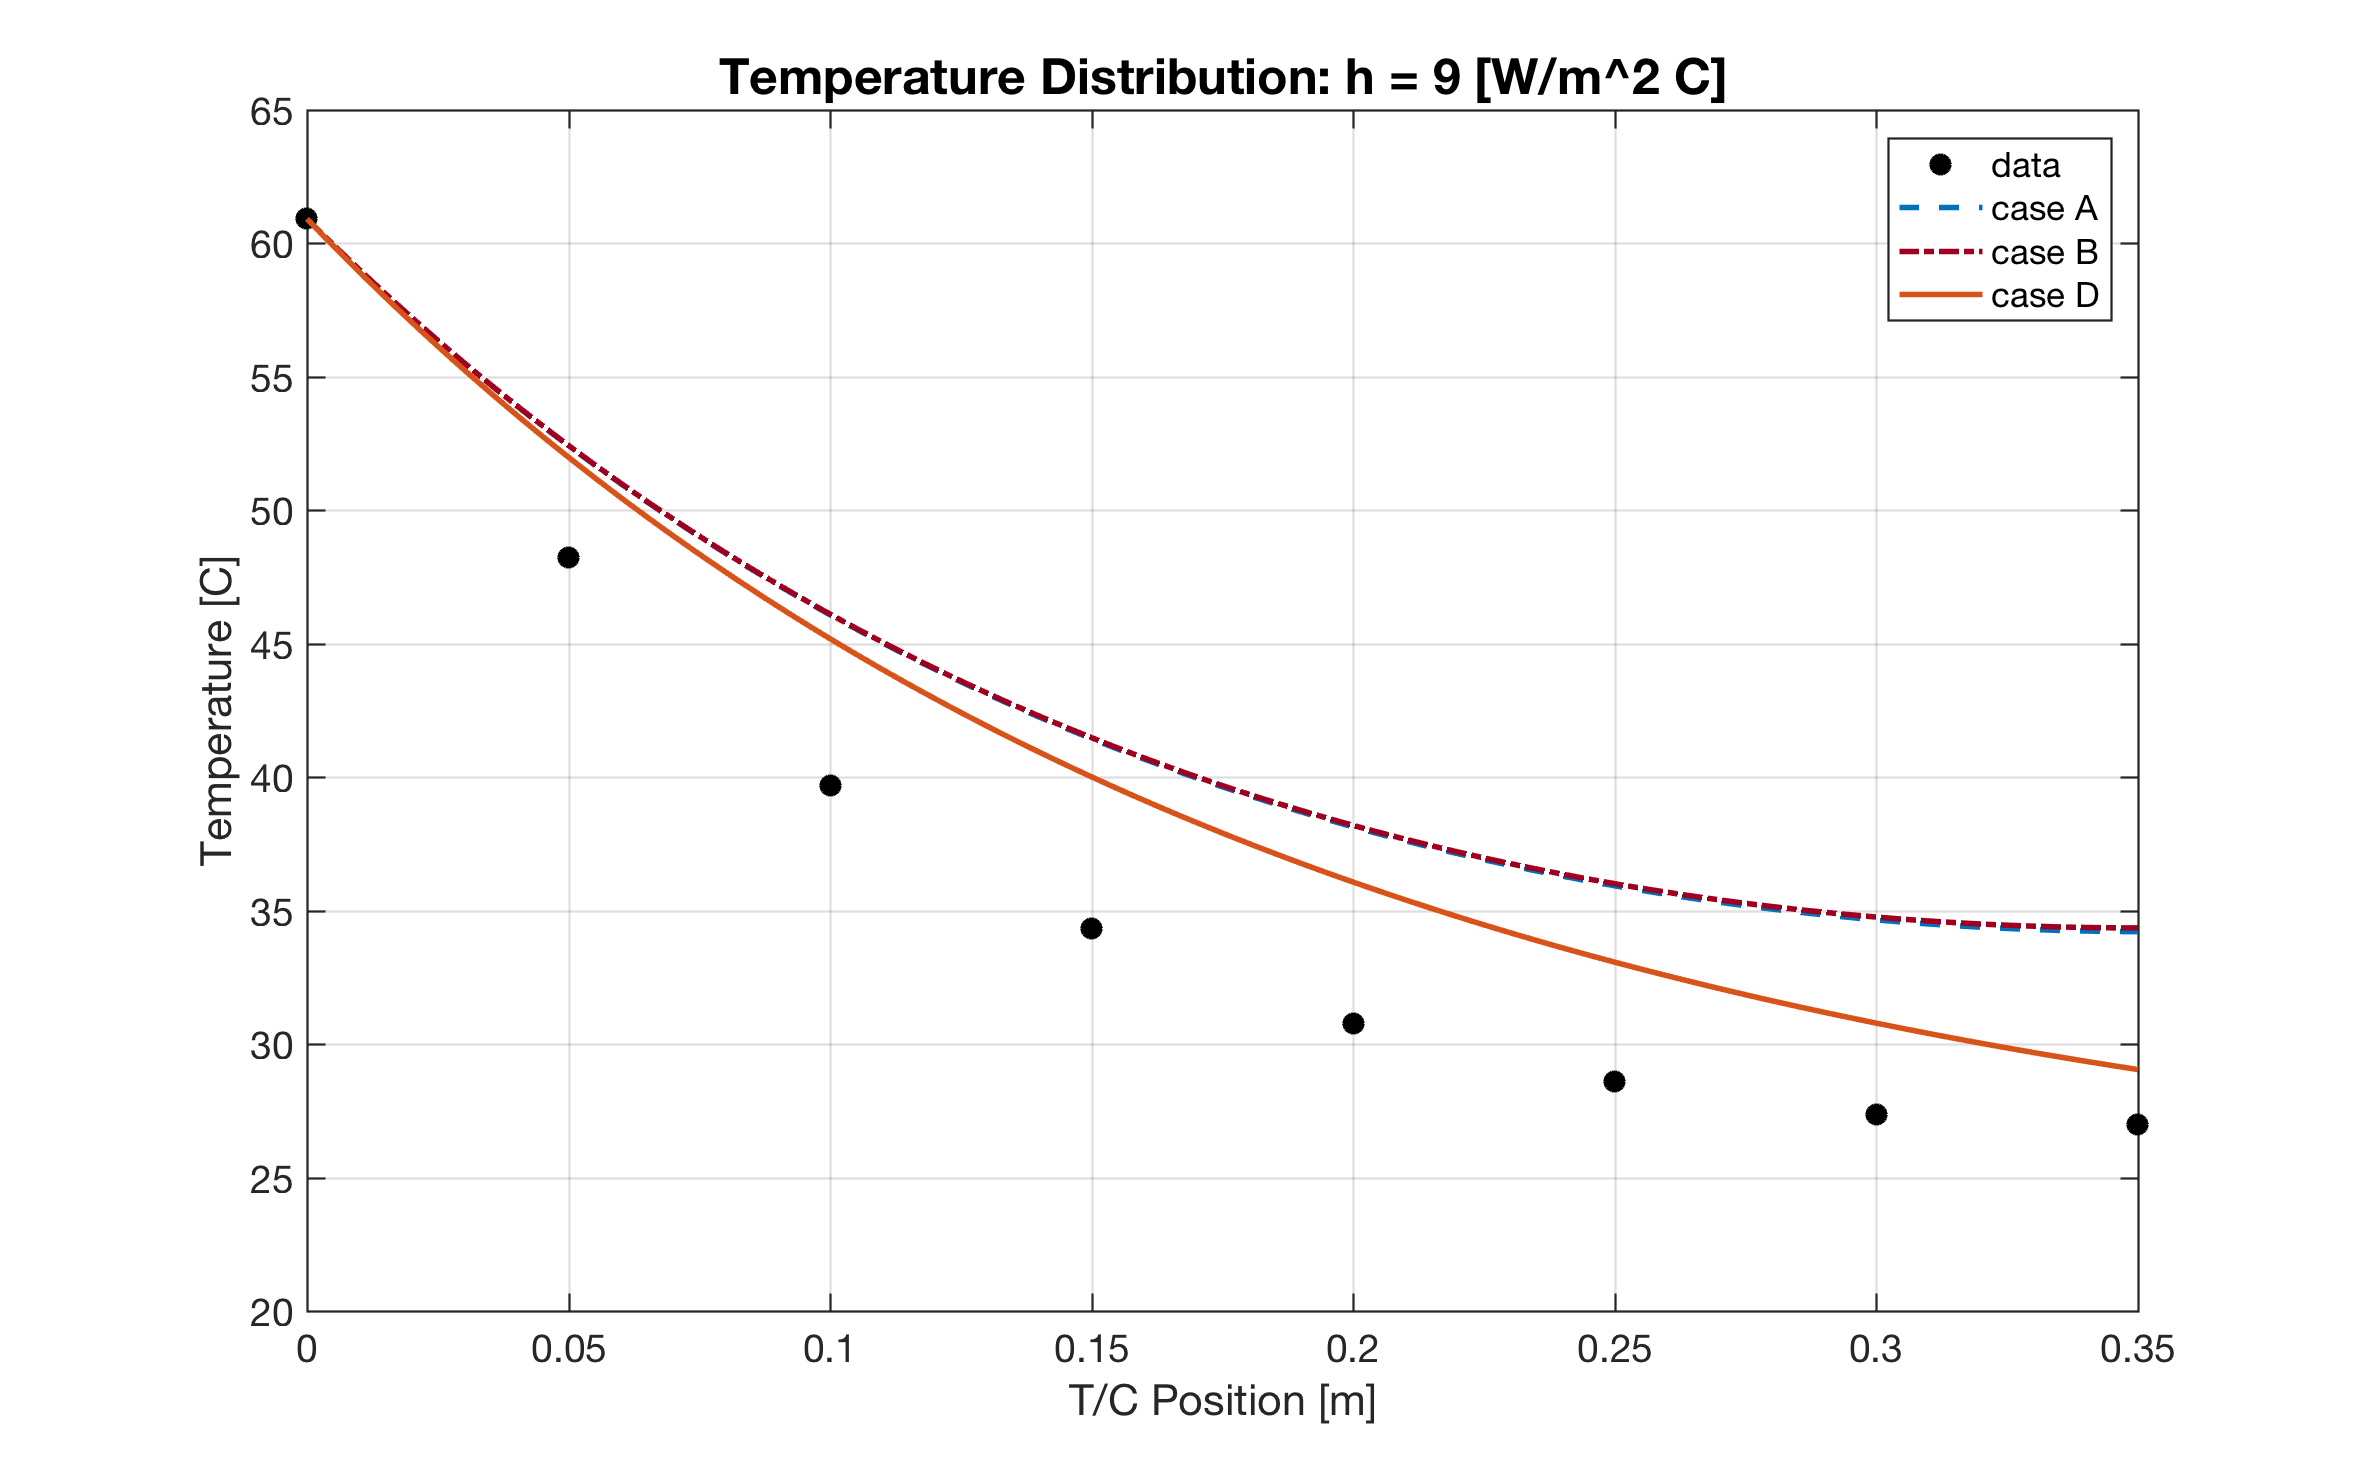
\includegraphics[width=125mm]{gfx/h09.png}
    \caption{Natural Convection: h = 9 $(W/m^2 C)$}\label{fig1}
    \end{center}
\end{figure}

\n
In addition, your code should have printed several lines to the command line. To gauge whether your code is correct, you should have:

\begin{lstlisting}[numbers=none]
 Effectiveness [-]:
 
    Station    CaseA     CaseB     CaseD 
    _______    ______    ______    ______
    '1'        70.264    70.181    73.333
    '3'        40.095    40.091    40.166
    '5'        34.764    34.763    34.785

\end{lstlisting}


\n
\section{Export Figures \& Deliverables}
In the \texttt{./figs} folder, you should see several images that have been exported automatically. These should be inserted into your report, rather than a screenshot. In addition, the tables have been exported as \texttt{.csv} files in the \texttt{./output} folder. You can simply copy/paste these into a nice Excel table for proper presentation.

\begin{formal}
    \begin{deliv} \bit{Export Figures:  } 
In a word processor (\it{MS Word, Pages, Open Office, or equivalent}) insert the three PNG images that you just produced  (\it{i.e.,} \texttt{h\_09.png, h\_30.png, h\_40.png}).  Then, \bit{write 1-2 sentences} describing the similarities/differences between each figure.
    \end{deliv}
\end{formal}

\begin{formal}
    \begin{deliv} \bit{Cmd Output:  } 
Next, copy/paste the output from the MATLAB Command Window  (\it{i.e.,} the tables showing Heat rate, error, efficiency, and effectiveness)
    \end{deliv}
\end{formal}

Once these deliverables are completed, print out your document and hand it in at the beginning of class.

\n
\hrule

\section{Radiation (Optional)}

This section is optional and will not be graded as part of the pre-lab assignment. However, since we will be using it throughout the experiment (and for your report), it has been included. 
\n

In this experiment, we are primarily interested in studying the effects of conduction and convection for an \it{extended surface}. That is, heat is transferred through the extended rod via conduction, and is presumed to be dissipated via convection. However, we know that radiation always plays a large role in this too. The question we now seek to answer is \bit{how large} of a role does radiation play? Particularly in relation to \it{convection}. In the sections that follow, we will estimate and compare the heat dissipated via convection and radiation for each of the experiment setups studied above.

\n
\subsection{Background: Radiation}

First, we take a look at the experiment through the lens of an infrared camera, as seen below:



\begin{figure}[H]
    \begin{center}
        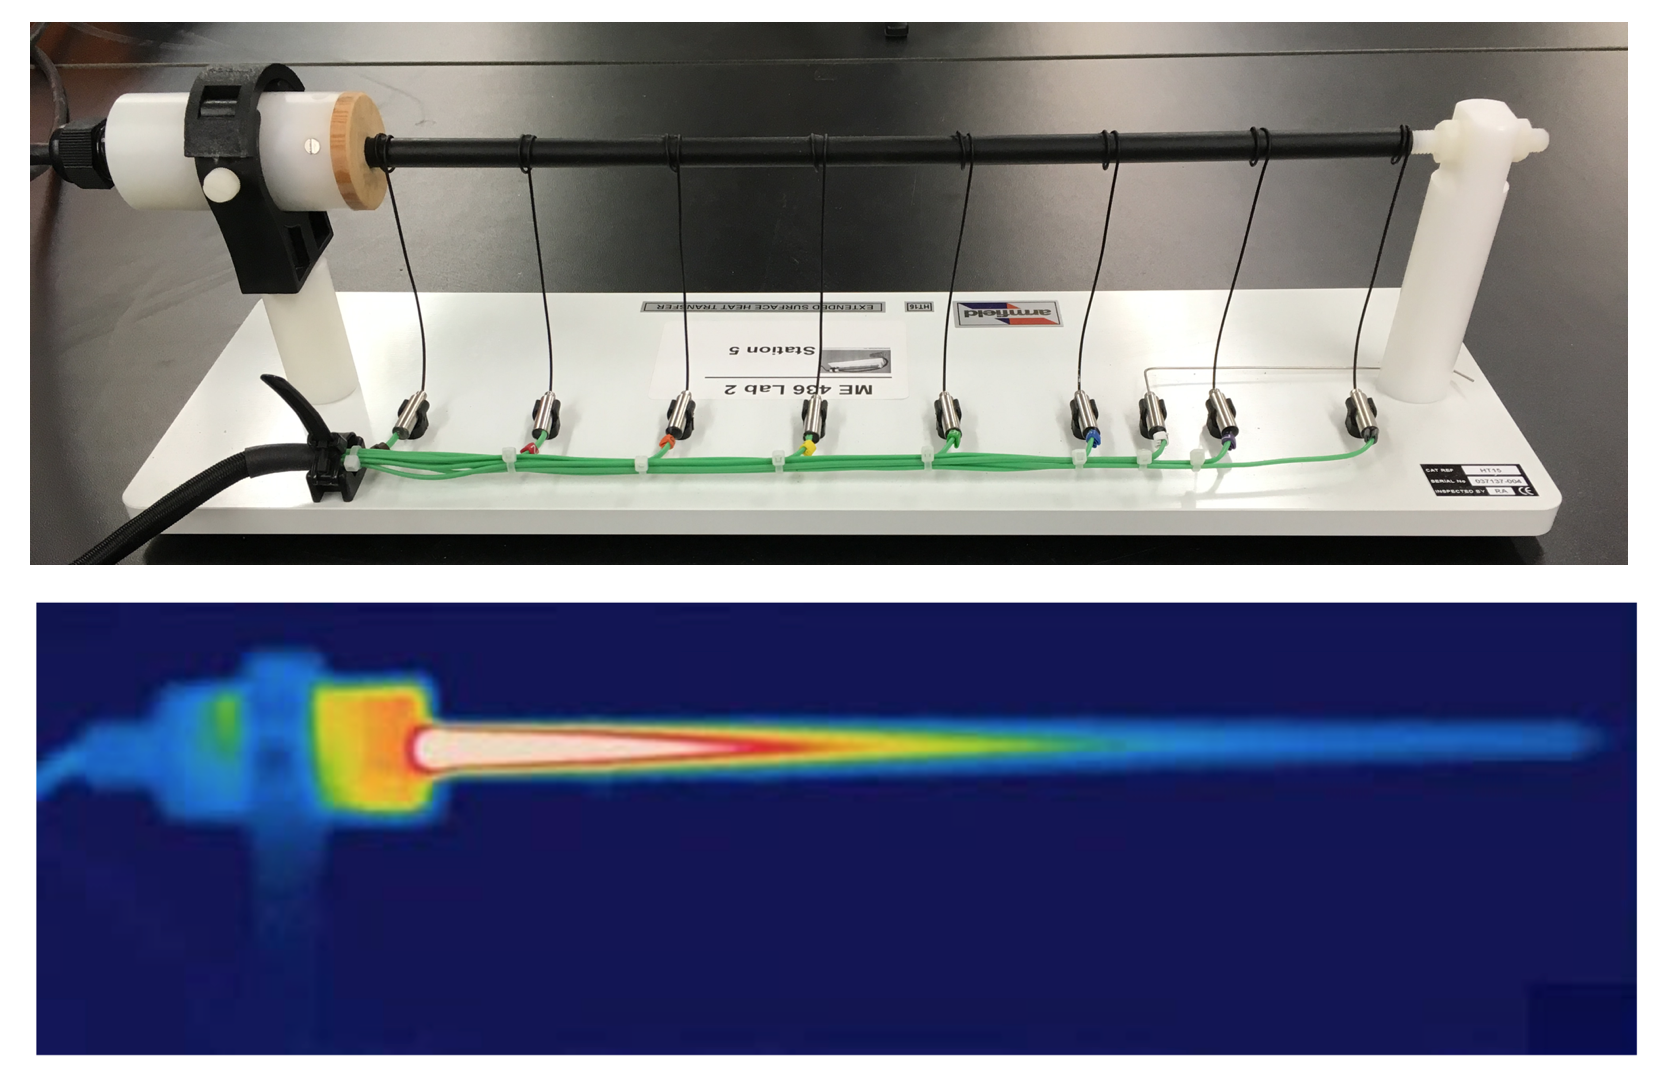
\includegraphics[width=125mm]{gfx/FLIR.png}
    \caption{FlIR Camera output}\label{fig2}
    \end{center}
\end{figure}

\n
This image shows us that we are dissipating a considerable amount of heat near the LHS of the apparatus; particularly along the first three thermocouples. In order to quantify this heat dissipation, lets make a few `\it{back of the envelope}' estimates.

\n
First, lets assume that radiation may be reasonably computed using the following equation:
\begin{equation}
q_{rad} = \epsilon \sigma A_s ( T_{avg}^4 - T_\infty^4 ) \ . \label{Eq1}
\end{equation}

\n
In which, $\sigma = \SI{5e-5}{(\watt\cdot\meter^{\text{-}2}\cdot\kelvin^{\text{-}4})} $, is the Stefan-Boltzmann constant, $\epsilon$ is the emissivity, $A_s$, the surface area, and $T_{avg}$, is the average material temperature, and $T_\infty$ refers to the surroundings (all units are standard metric).
\n
Now, since the \it{heat rate}, $q$, is essentially the integral of our temperature distribution over a given area, lets make \it{broad stroke} estimates for $A_s$ and $T_{avg}$: lets use an average temperature $T_{avg}$, collected over an area covering only the first \bul{ $1/3$ of the rod length.} This is easily done using the `\it{boxed averaging}' tool included with the FLIR Camera Toolset. Concretely, we assume $A_s$ is computed by:
\eq{
A_s = \pi D ( \sfrac{1}{3} L ) \ .
}
\n
When using the FLIR camera, isolating only this section gives us more confidence in our $T_{avg}$ value, rather than averaging over the length of the rod. In addition, this allows us to use the simplified equation above, which only uses an averaged temperature, $T_{avg}$.

\begin{figure}[H]
    \begin{center}
        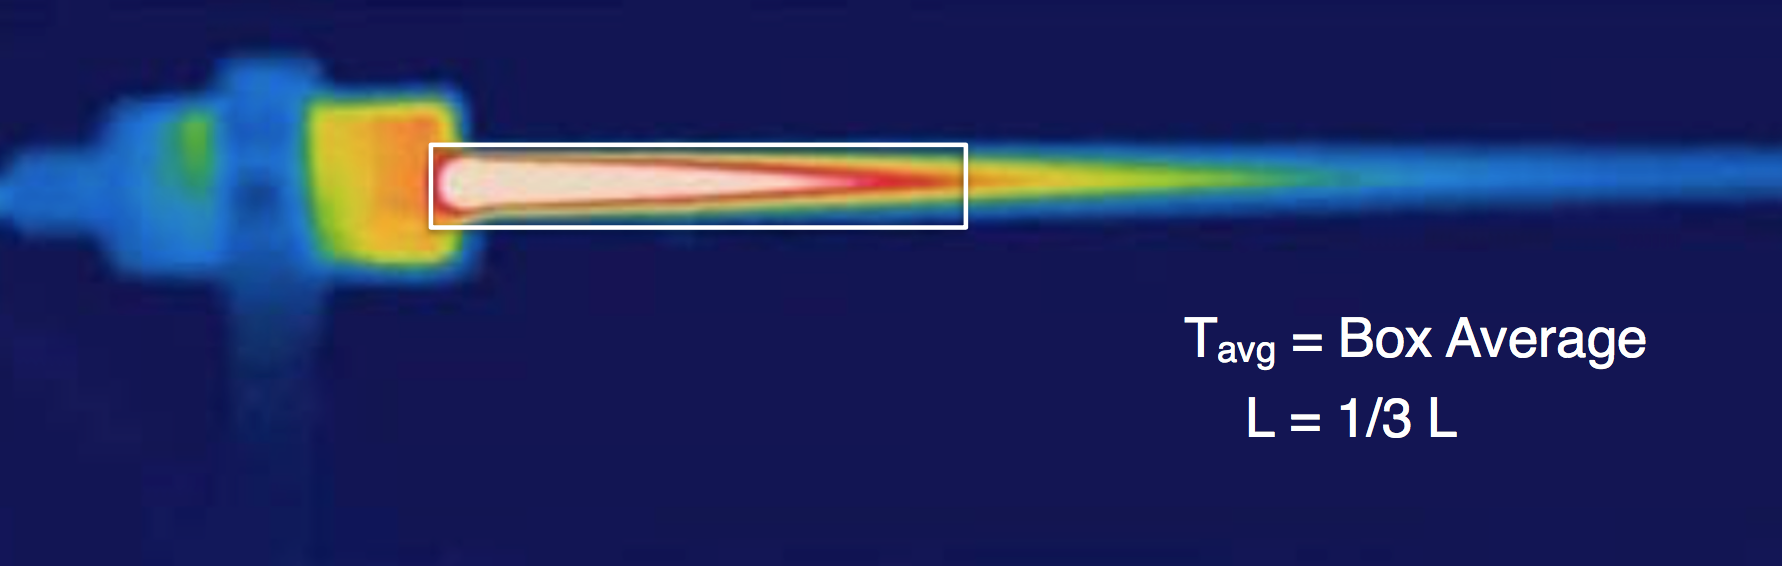
\includegraphics[width=125mm]{gfx/FLIR2.png}
    \caption{FlIR Tools: Boxed Averaging}\label{fig3}
    \end{center}
\end{figure}

If we were to sketch this out on paper, our estimate would look similar to the image below.

\begin{figure}[H]
    \begin{center}
        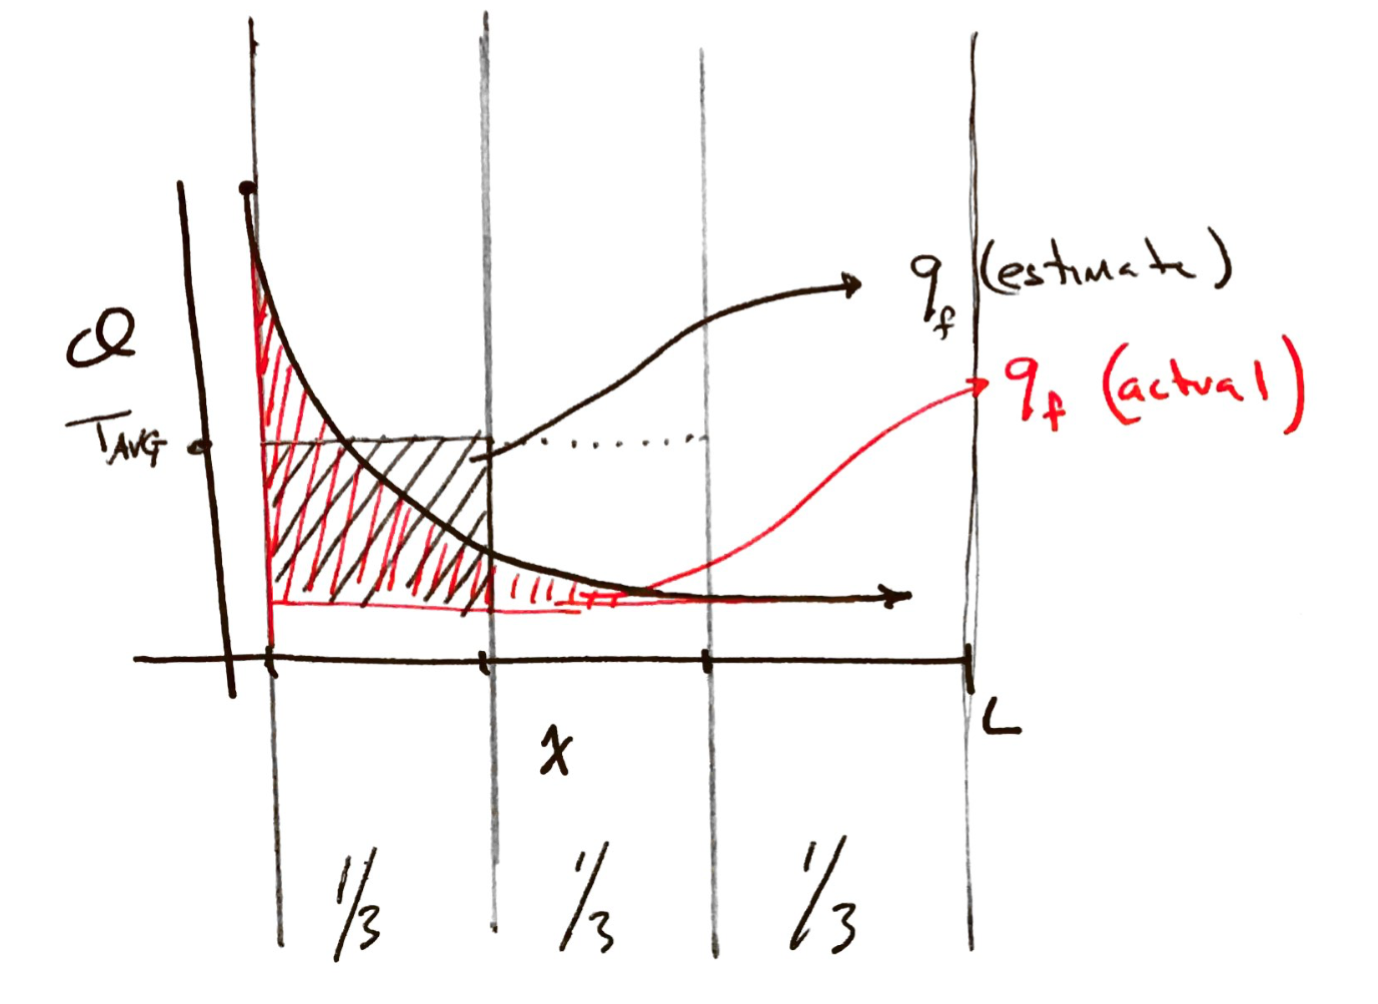
\includegraphics[width=90mm]{gfx/sketch.png}
    \caption{Estimated heat rate}\label{fig4}
    \end{center}
\end{figure}

As you can see here, the \it{actual} temperature distribution is an exponential curve. While we could integrate this numerically (since we have the FLIR data), at the moment we're only interested in a quick \it{estimate}. Hence, the above approximation should be sufficient.

\n
\subsection{Background: Convection}

Now, since we have assumed that all other losses are negligible (\it{i.e.,} conduction, uncertainty in system \&, \it{etc.}), we can use the same arguments made above to estimate the losses due to convection. That is, lets assume that the following equation is sufficient:
\begin{equation}
q_{conv} = h A_s ( T_{avg} - T_\infty ) \ .\label{Eq2}
\end{equation}

\n
In which $ A_s = \pi D ( \sfrac{1}{3} L )$, $h$ is the convection coefficient, $T_{avg}$ is again our \it{box-averaged} temperature. 

\n
\subsection{Implementation}

Now, let's implement the above in MATLAB. When completed, you should have a bar graph that resembles:

\begin{figure}[H]
    \begin{center}
        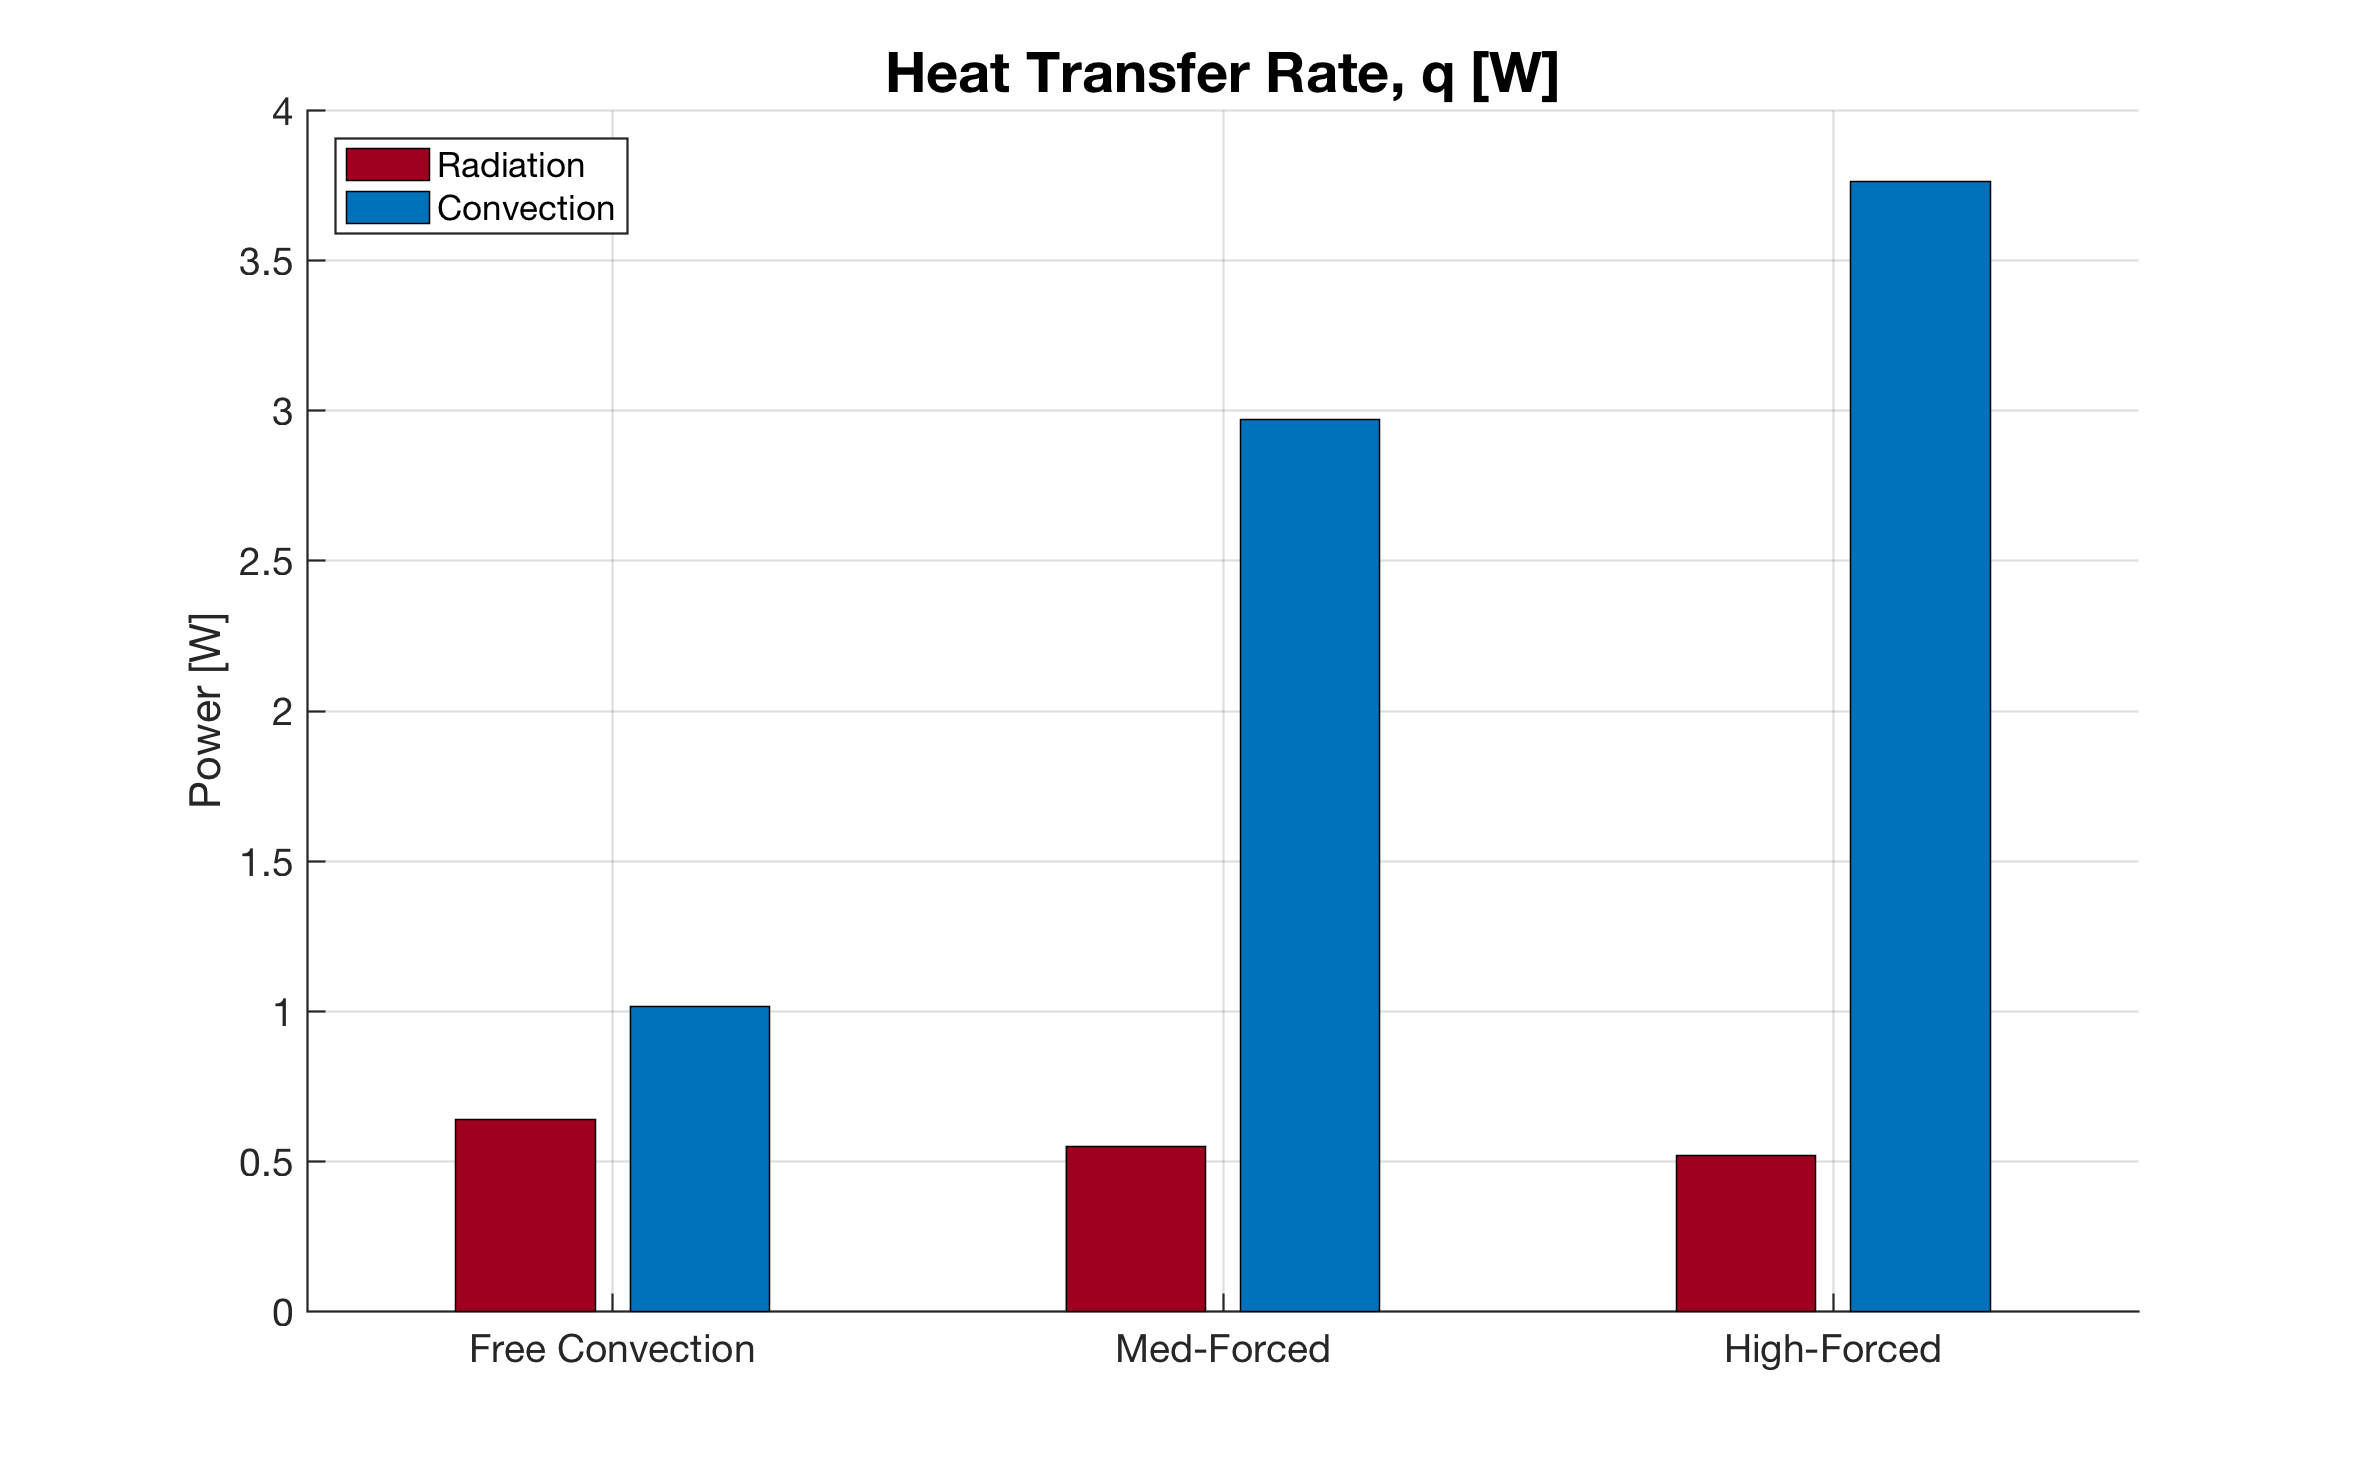
\includegraphics[width=120mm]{gfx/rad_estimation.png}
    \caption{Estimated heat rate for each station}\label{fig5}
    \end{center}
\end{figure}

\n
First, open the file \bd{\texttt{ex2\_rad.m}}. As before, make sure the script can find your data. Be sure that your paths are as well as the properties.

Note, you will need to make adjustments to emissivity as more information comes available to you. For instance, using the FLIR camera to extract a accurate value vs. using an estimation from the textbook.
\begin{lstlisting}[numbers=none]
% calibrated ep from FLIR camera (0.78 - 0.82)
ep = 0.82;

% Set Tinf -- as measured in lab
Tinf = 23.5 + 273;     % [K]
\end{lstlisting}

When performing the experiment, you will need to adjust the ambient air temperature, $T_{\inf}$ as well as the emissivity (information on this will be provided at a later point -- for now, the default value will work fine).

\n

Now, we begin the loop over all data sets.
\begin{lstlisting}[numbers=none]
% loop over stations
for ii = 1:length(fname)
...
\end{lstlisting}

\n
The only lines that you need to be concerned with are the following:

\begin{lstlisting}[numbers=none]
% radiation & convection estimations
q_rad(ii) = calc_rad(T);
q_conv(ii)= calc_conv(T,h(ii));
\end{lstlisting}

To get this working, you need to open \bd{\texttt{calc\_rad.m}} \& \bd{\texttt{calc\_conv.m}} and insert Eq. \ref{Eq1} \& Eq. \ref{Eq2} (above), respectively. If executed correctly you should obtain Fig. \ref{fig5} above, as well as the following command line output:

\n
\begin{lstlisting}[numbers=none]
 Heat Transfer Rate [W]:
 
    Station    CONV      RAD     PCT_RAD
    _______    _____    _____    _______
    'Free'     1.015    0.639    38.6   
    'Med'      2.971     0.55    15.6   
    'High'     3.764     0.52    12.1 
\end{lstlisting}

\subsection{Conclusions}

Tabulating the above results, we can now clearly see the relative impact of neglecting radiation for each station. The apparent trend is that as the convection coefficient increases, radiation plays a lesser role

\definecolor{Gray}{gray}{0.95}
\newcolumntype{g}{>{\columncolor{Gray}}c}
\begin{center}
{\small
\begin{tabular}{l|ccg}
Station & Conv. [W] & Rad. [W] & Pct Rad. \\ [0.25em]
  \hline
  \it{Free} & 1.0  & 0.7 & \bit{38.6} \% \\
  \it{Med} & 3.0 & 0.6  & \bit{15.6} \% \\
  \it{High} & 3.8 & 0.5 & \bit{12.1} \%
\end{tabular}
}
\end{center}

\n

\begin{formal}
    \begin{deliv} \bit{In-class assignment } 
Based upon the results above is it acceptable to neglect radiation for any of the above cases? Justify your answer.
    \end{deliv}
\end{formal}


\end{document}
